\documentclass[autodetect-engine,dvipdfmx-if-dvi,ja=standard,a4j,jbase=11pt,magstyle=nomag*]{bxjsreport}
% \documentclass[uplatex, dvipdfmx, a4paper, 11ptj, report]{jsbook}
% small japanese font size:     9pt, 10pt, 11pt, 12pt, 14pt, ... (please refer the document of jsclasses)
% word-like japanese font size: 10ptj 10.5ptj, 11ptj, 12ptj (or jbase=xxpt (without 'j') if error is occured)

\usepackage{ifptex,ifxetex,ifluatex}
\ifluatex
    \usepackage{bxcalcux}
    \ltjsetparameter{jacharrange={-2,-3}}
    \usepackage{luatexja-otf}
    \usepackage{bxbase}
\else\ifxetex
    % \usepackage{zxjatype}
    % \usepackage[macros]{zxotf}
    \XeTeXgenerateactualtext=1
    \usepackage{xltxtra}
    \usepackage{bxbase}
\else\ifuptex
    \usepackage{otf}
    \usepackage[prefernoncjk]{pxcjkcat}
    \cjkcategory{sym11,sym18,sym19}{cjk}
    \usepackage[utf8]{inputenc}
    \usepackage{pxbase}
\else\ifstrictptex
    \usepackage{otf}
    \usepackage[utf8]{inputenc}
    \usepackage{pxbase}
\fi\fi\fi\fi

\usepackage[LGR,T2A,T1]{fontenc}

\usepackage{graphicx}
% \usepackage[dvipdfmx]{graphicx}
\usepackage{grffile}

% paper layout setting
\setpagelayout{noheadfoot, left=18.0truemm, right=18.0truemm, top=29.0truemm, bottom=26.0truemm, columnsep=6.5truemm}
% \setpagelayout{noheadfoot, left=15.0truemm, right=5.0truemm, top=12.5truemm, bottom=12.5truemm, columnsep=5.0truemm}

% font setting
\usepackage{amsmath}
\usepackage{amssymb}
\usepackage{mathtools}
\usepackage{bm}
\usepackage{fix-cm}
\usepackage{newtxtext}
\usepackage[slantedGreek]{newtxmath}

% caption setting
\usepackage[font=bf,labelfont=bf,labelsep=quad]{caption}

% to balance the last page of the two-column article
% \usepackage[nospread, keeplastbox, nodebug]{flushend}

% title font style
\renewcommand{\headfont}{\bfseries}

% section setting (using titlesec, uelm package)
\renewcommand{\thesection}{\arabic{section}}
\renewcommand{\thesubsection}{\arabic{section}.\arabic{subsection}}

\usepackage[explicit]{titlesec}
\usepackage[normalem]{ulem}
\titleformat{name=\section}{\normalfont\headfont\normalsize\raggedright}{}{0pt}{\uline{\thesection.\quad#1}}
\titleformat{name=\section,numberless}{\normalfont\headfont\normalsize\raggedright}{}{0pt}{\uline{#1}}
% \titleformat{name=\section}{\normalfont\headfont\normalsize\raggedright}{}{0pt}{\thesection.\quad#1}
\titlespacing{name=\section}{0pt}{.5\Cvs plus .0\Cvs minus .3\Cvs}{.1\Cvs plus .0\Cvs minus .1\Cvs}
\titleformat{name=\subsection}{\normalfont\headfont\normalsize\raggedright}{}{0pt}{\thesubsection.\quad#1}
\titleformat{name=\subsection,numberless}{\normalfont\headfont\normalsize\raggedright}{}{0pt}{#1}
\titlespacing{name=\subsection}{0pt}{.3\Cvs plus .0\Cvs minus .2\Cvs}{.0\Cvs plus .0\Cvs minus .0\Cvs}

% \makeatletter
% \renewcommand{\section}{\@startsection{section}{1}{\z@}{.5\baselineskip}{.1\baselineskip}{\normalfont\normalsize\headfont\raggedright}}
% \renewcommand{\subsection}{\@startsection{subsection}{2}{\z@}{.3\baselineskip}{\z@}{\normalfont\normalsize\headfont\raggedright}}
% \makeatother

\usepackage{secdot}
\sectiondot{section}
\sectiondot{subsection}

% list (itemize, enumerate, description, ...)
\usepackage{enumitem}
\setlist[1]{parsep=.0\baselineskip,topsep=.2\baselineskip,itemsep=.1\baselineskip}
% \makeatletter
% \def\@listi{\leftmargin\leftmargini
%     \parsep \z@
%     \topsep .2\baselineskip
%     \itemsep .1\baselineskip \relax}
% \let\@listI\@listi
% \makeatother

% no page number
\pagestyle{empty}

% footnote
\usepackage[bottom,hang,stable]{footmisc}
\setlength{\footnotemargin}{0pt}

% float setting (figure, table)
\setlength\floatsep{2.0truemm}
\setlength\textfloatsep{2.0truemm}
\setlength\intextsep{1.0truemm}
\setlength\dblfloatsep{2.0truemm}
\setlength\dbltextfloatsep{2.0truemm}
\setlength\abovecaptionskip{0.5truemm}
\setlength\belowcaptionskip{0.5truemm}

% lineskip setting (body text, display-style equation)
\AtBeginDocument{%
    \narrowbaselines    % basic english lineskip (for article)
    % \widebaselines      % basic japanese lineskip
    %
    \setlength\abovedisplayskip{1.5truemm}    % equation setting
    \setlength\belowdisplayskip{1.5truemm}    % equation setting
}

% to suit ms-word template
\renewcommand{\baselinestretch}{0.9}


\makeatletter
%
% maketitle
% additional elements
\newcommand*{\etitle}[1]{\gdef\@etitle{#1}}
\newcommand*{\studentid}[1]{\gdef\@studentid{#1}}
\newcommand*{\laboarea}[1]{\gdef\@laboarea{#1}}
\newcommand*{\laboname}[1]{\gdef\@laboname{#1}}
%
% style definition
\def\@maketitle{%
\newpage%
\centering%
\let\footnote\thanks%
%
% title
{\fontsize{16.00truept}{16.00truept}\selectfont\headfont\@title\par}%
%
% english title
\ifx\@etitle\@undefined\else{\vspace{1truemm}{\fontsize{12truept}{12truept}\selectfont\headfont\@etitle\par}}\fi%
%
% name (option: student id)
\vspace{1truemm}%
\ifx\@studentid\@undefined\else{\fontsize{12truept}{12truept}\selectfont\headfont\@studentid\hspace{\Cwd}}\fi%
{\fontsize{12truept}{12truept}\selectfont\headfont\@author\par}%
%
% research area (\laboarea) and laboratory name (\laboname)
\ifx\@laboarea\@undefined%
    \ifx\@laboname\@undefined%
    \else\vspace{1truemm}{\fontsize{12truept}{12truept}\selectfont\headfont\@laboname\par}%
    \fi%
\else%
    \ifx\@laboname\@undefined\vspace{1truemm}{\fontsize{12truept}{12truept}\selectfont\headfont\@laboarea\par}%
    \else\vspace{1truemm}{\fontsize{12truept}{12truept}\selectfont\headfont\@laboarea\hspace{\Cwd}\@laboname\par}%
    \fi%
\fi%
%
%% old version (2 line) of research area (\laboarea) and laboratory name (\laboname)
%\ifx\@laboarea\@undefined\else{\vspace{1truemm}{\fontsize{10truept}{10truept}\selectfont\@laboarea\par}}\fi%
%\ifx\@laboname\@undefined\else{\vspace{1truemm}{\fontsize{10truept}{10truept}\selectfont\@laboname\par}}\fi%
%
%% date (error)
% \ifvoid\@date\else{\vspace{2truemm}{\fontsize{12truept}{12truept}\selectfont\@date\par}}\fi%
%
% abstract (no check)
\ifvoid\@abstractbox\else{\vspace{2truemm}{\centering{\fontsize{10truept}{10truept}\selectfont\box\@abstractbox\par}}}\fi%
\vspace{2truemm}%
}
%
%
% bibliography
\newcommand{\@bibsection}{\@startsection{section}{1}{\z@}{.5\baselineskip}{0.2\baselineskip}{\normalfont\fontsize{9truept}{11truept}\selectfont\headfont\raggedright}}
\setlength\bibindent{\Cwd}
\renewenvironment{thebibliography}[1]{%
    \global\let\presectionname\relax
    \global\let\postsectionname\relax
    \@bibsection*{\refname}\@mkboth{\refname}{\refname}%
    \list{\@biblabel{\@arabic\c@enumiv}}{%
        \settowidth\labelwidth{\@biblabel{#1}}%
        \leftmargin\labelwidth
        \advance\leftmargin\labelsep
        \setlength\itemsep{0.5truept plus 1.0truept minus 0.5truept}
        \@openbib@code
        \usecounter{enumiv}%
        \let\p@enumiv\@empty
        \renewcommand\theenumiv{\@arabic\c@enumiv}}%
    \fontsize{8truept}{9.5truept}\selectfont
    \sloppy
    \clubpenalty4000
    \@clubpenalty\clubpenalty
    \widowpenalty4000%
    \sfcode`\.\@m}
{\def\@noitemerr{\@latex@warning{Empty `thebibliography' environment}}\endlist}
%
\makeatother


\mainmatter
\setchapterxr[thesis][bibliography]{3}


\begin{document}


\chapter[複数LiDARの位置校正方法とオクルージョン範囲を考慮した撮影計画]{複数LiDARの位置校正方法と\\オクルージョン範囲を\\考慮した撮影計画}
	
\section{はじめに}
本章では,LiDARの位置を取得するために使用した手法を説明する.
また,決定したLiDARの位置とそれが認識した人物の位置からオクルージョンが起こっている範囲を導出し,
その範囲をUAVが撮影できるように目標位置を設定する手法を説明する.

\section{複数LiDARの位置決定方法}
まず始めに,複数LiDARの位置の取得方法について述べる.
先行研究では1台のLiDARの位置をUAVに搭載しているGPSセンサと同じもの使用してを取得していた.
しかし,UAVに搭載されているGPSセンサから得られる緯度経度情報は数mから十数mの誤差がある.
複数のLiDARを使用する際,位置の誤差が大きいと,1つの物体を2つの物体と誤認してしまう恐れがある.
そのため,2つのLiDARの正確な相対位置を取得するためにRTK-GPS測位という手法を利用して位置を取得する.

\subsection{RTK-GPS測位}
RTK-GPS(Real-Time Kinematic GPS)測位とは,位置が分かっていて移動しない基地局(Base)と
位置情報を取得しようとしている観測点である移動局(Rover)で同時にGPS観測を行い,
基準局で観測したデータを移動局へリアルタイムに送信し,基準局の位置に基づいて移動局の位置を求める手法である.
さらにネットワークを利用して基地局と移動局のデータ送信を行うことで,
基地局と移動局が長距離で離れていても精度の高い演算ができる.

\begin{figure}[t]
    \centering
    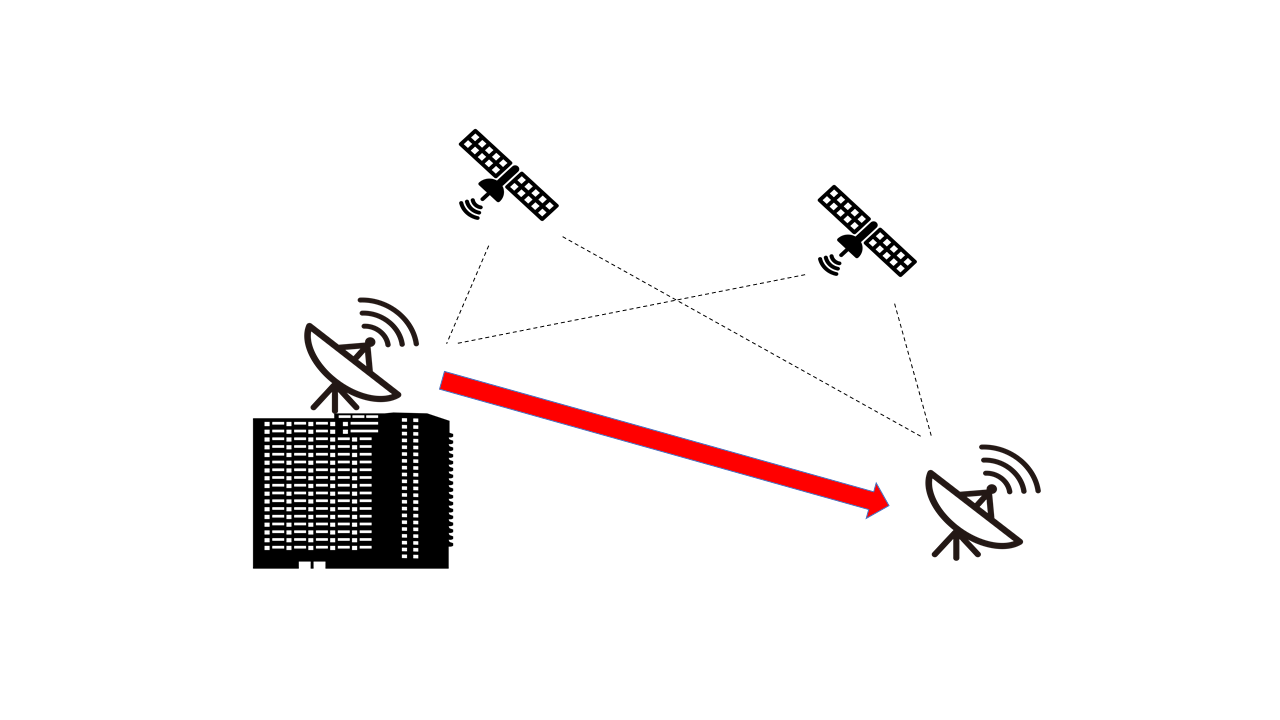
\includegraphics[width=\linewidth, clip]{./figure/chapter3/RTK.png}
    \caption{Image of RTK-GPS Positioning System}
    \label{fig:RTK}
\end{figure}

\subsection{RTK-GPS測位と単独測位の比較}
単独測位では数mから十数mの誤差が発生するのに対して,
RTK-GPS測位では数cmの誤差が発生するといわれている.
ここで,実際に計測したデータを比較して測位の性能の差を述べる.
計測位置は大阪市立大学F棟507号室のベランダであり,\cref{fig:data_of_RTK}は30秒の計測データをグラフ化したものである.
\cref{fig:data_of_RTK}左のグラフは単独測位の結果であり,グラフは1マス50cmである.
同図右のグラフはRTK-GPS測位の結果であり,グラフは1マス1cmである.
グラフはから見て取れるように,単独測位は50cmから1mの誤差があり,
RTK-GPS測位の誤差は1cmから2cm以内に収まっている.

\begin{figure}[t]
    \centering
    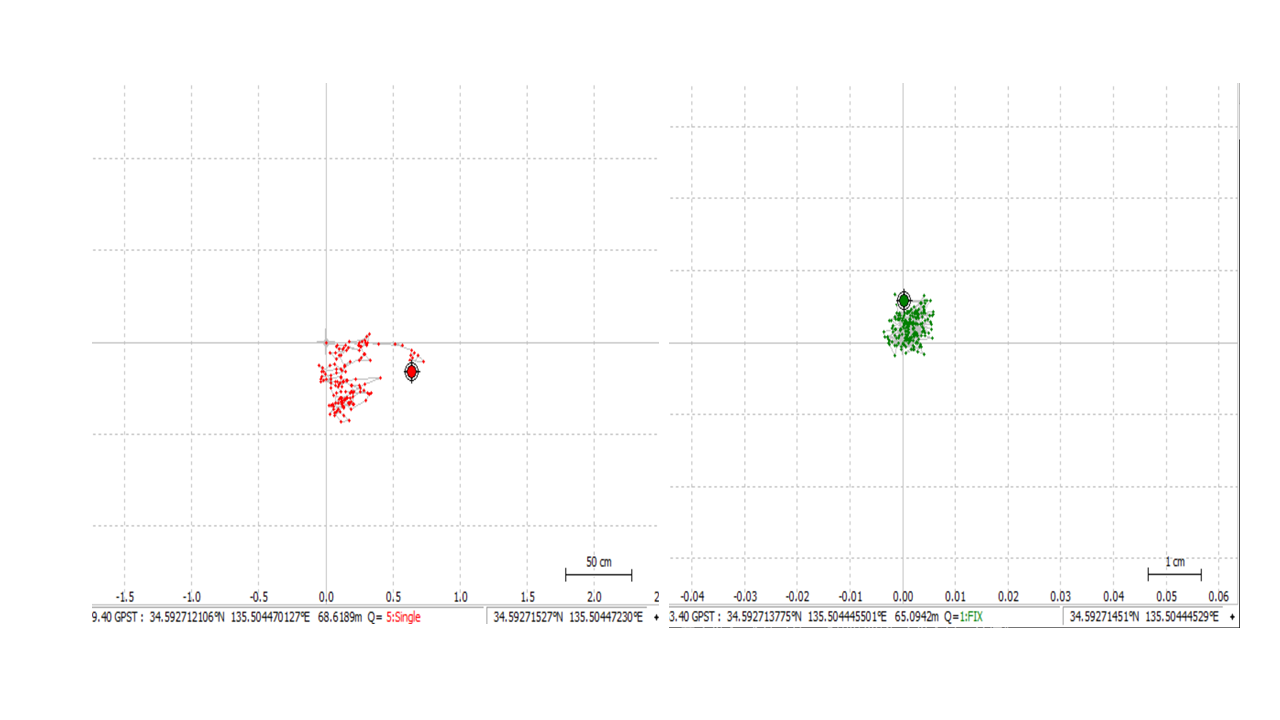
\includegraphics[width=\linewidth, clip]{./figure/chapter3/Data_of_GPS_positioning.png}
    \caption{Single GPS Positioning (right) and RTK-GPS Positioning (left)}
    \label{fig:data_of_RTK}
\end{figure}

\section{GPS座標からmap座標への変換}
本研究では,東を{\it x}座標正方向,北を{\it y}座標正方向とするmap座標系を用いる.
また座標原点はLiDAR1の座標をもとに算出する.
ここでは,GPSセンサから得たLiDAR1の緯度経度と座標から原点の緯度経度の値の算出方法,
原点の緯度経度の値とLiDAR2の緯度経度の値からLiDAR2のmap座標の算出方法を述べる.

LiDAR1のGPS座標を$lon_{lidar1}, lat_{lidar1}$,map座標を$x_{lidar1}, y_{lidar1}$とすると
求めるmap座標原点の緯度経度の値$lon_{origin}, lat_{origin}$は以下の\cref{eq:calc_gps}で算出される.
なお式中の$R$は地球の赤道半径である.

\begin{equation}
    \begin{aligned}
        lat_{origin} &= \frac{y_{lidar1}}{R} \times \frac{180}{\pi} + lat_{lidar1}\\
        lon_{origin} &= \frac{x_{lidar1}}{R} \times \frac{180}{\pi} \times \frac{1}{cos( lat_{origin} \frac{180}{\pi})} + lon_{origin}
    \end{aligned}
    \label{eq:calc_gps}
\end{equation}

\cref{eq:calc_gps}より得られたmap座標原点の緯度経度の値を用いて,
LiDAR2のmap座標$x_{lidar2}, y_{lidar2}$を\cref{eq:calc_from_gps}求めることができる.
LiDAR2のGPS座標を$lon_{lidar2}, lat_{lidar2}$とする.

\begin{equation}
    \begin{aligned}
        x_{lidar2} &=  R ( lon_{lidar2} - lon_{lidar2} ) \frac{\pi}{180} cos(( lat_{lidar2} - lat_{origin} )\frac{\pi}{180}) \\
        y_{lidar2} &=  R ( lat_{llidar2} - lat_{origin} ) \frac{\pi}{180}
    \end{aligned}
    \label{eq:calc_from_gps}
\end{equation}

\section{オクルージョンが発生した場合のUAVの撮影位置の決定}
前節まででは,LiDARの位置を取得するための手法を述べた.
人物行動範囲内に複数人の人物が存在する場合,オクルージョンが発生し.
地上設置LiDARでは人物行動範囲内の全ての人物をとらえきれない場合が存在する.
この節では,オクルージョンが発生した場合のLiDARの撮影できない領域と,
その領域を考慮したUAVの目標位置の導出方法について述べる.

\subsection{1台のLiDARに対するオクルージョンの範囲}
LiDARの設置位置と人物の位置関係からLiDARが物体を認識することのできない領域を推定することができる.
この領域をオクルージョンエリアと定義する.
簡単のため人物の形を円形としその半径を$r$とすると\cref{fig:occlusion_area}で示される領域がオクルージョンエリアとなる.

\begin{figure}[t]
    \centering
    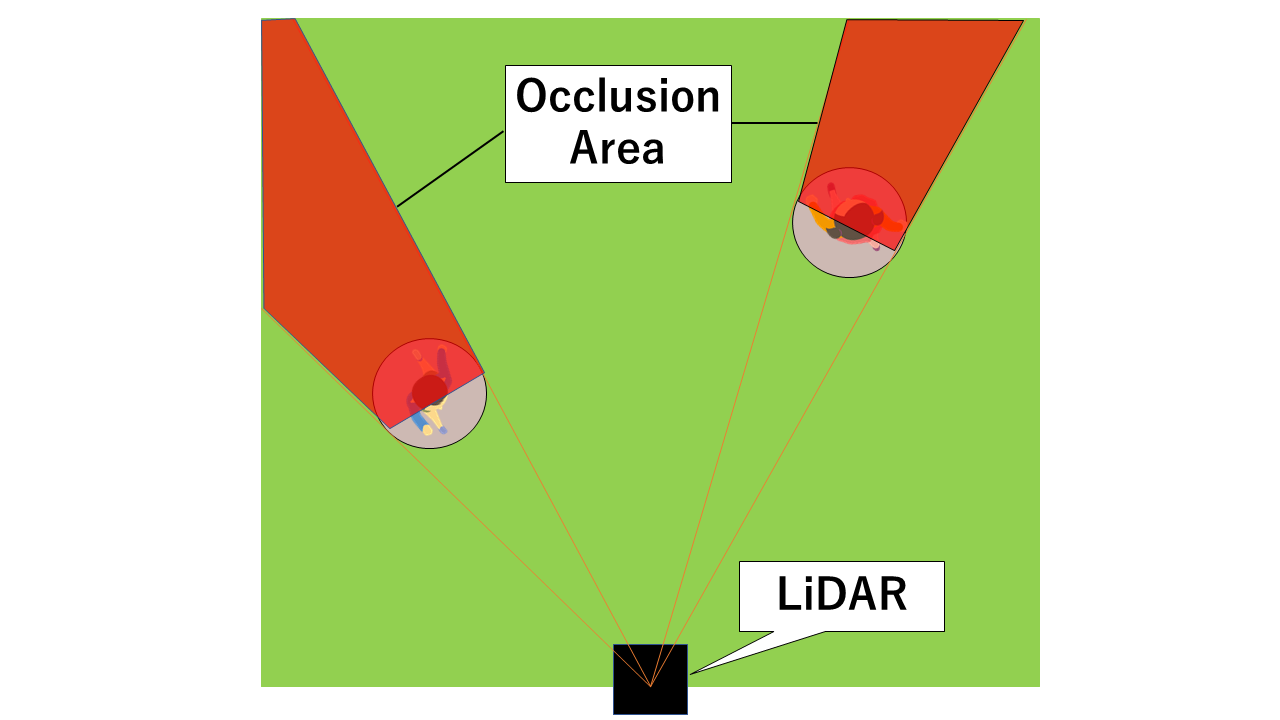
\includegraphics[width=\linewidth, clip]{./figure/chapter3/occlusion_area.png}
    \caption{Occlusion Area}
    \label{fig:occlusion_area}
\end{figure}

オクルージョンエリアは人物の円に対してLiDARの座標を通る2本の接線を考え,
2接点を結んだ線と2本の接線,人物の移動可能範囲の境界に囲まれる領域になる.
このオクルージョンエリアに人物が存在した場合,地上カメラから捉えられないためUAVが撮影する必要がある.
本研究では,オクルージョンエリアに架空の人物がいると想定して撮影計画を行う.
架空の人物(ダミー)の座標を設定することで,ダミーに対しても撮影ベクトルが付与され
オクルージョンエリアを撮影範囲に収めることができる.

ダミーの座標の位置は,LiDARと人物を表す円の中心座標を結ぶ直線と人物移動可能範囲の領域との交点を
導出し,その交点の座標と人物の円の中心座標の中点に設定する.
LiDARの座標を$x_{lidar}$,$y_{lidar}$,人物の円の中心座標を$x_{person}$,$y_{person}$とすると
2点を結ぶ直線の方程式は\cref{eq:occlusion}で求めることができる.
ここでは人物移動可能領域の中心を原点とする座標系を使用する.

\begin{equation}
    \begin{aligned}
       y = \frac{y_{person} - y_{lidar}}{x_{person} - x_{lidar}} x + 
\frac{x_{person}y_{lidar} - x_{lidar}y_{person}}{x_{person} - y_{lidar}}
    \end{aligned}
    \label{eq:occlusion}
\end{equation}

\begin{figure}[t]
    \centering
    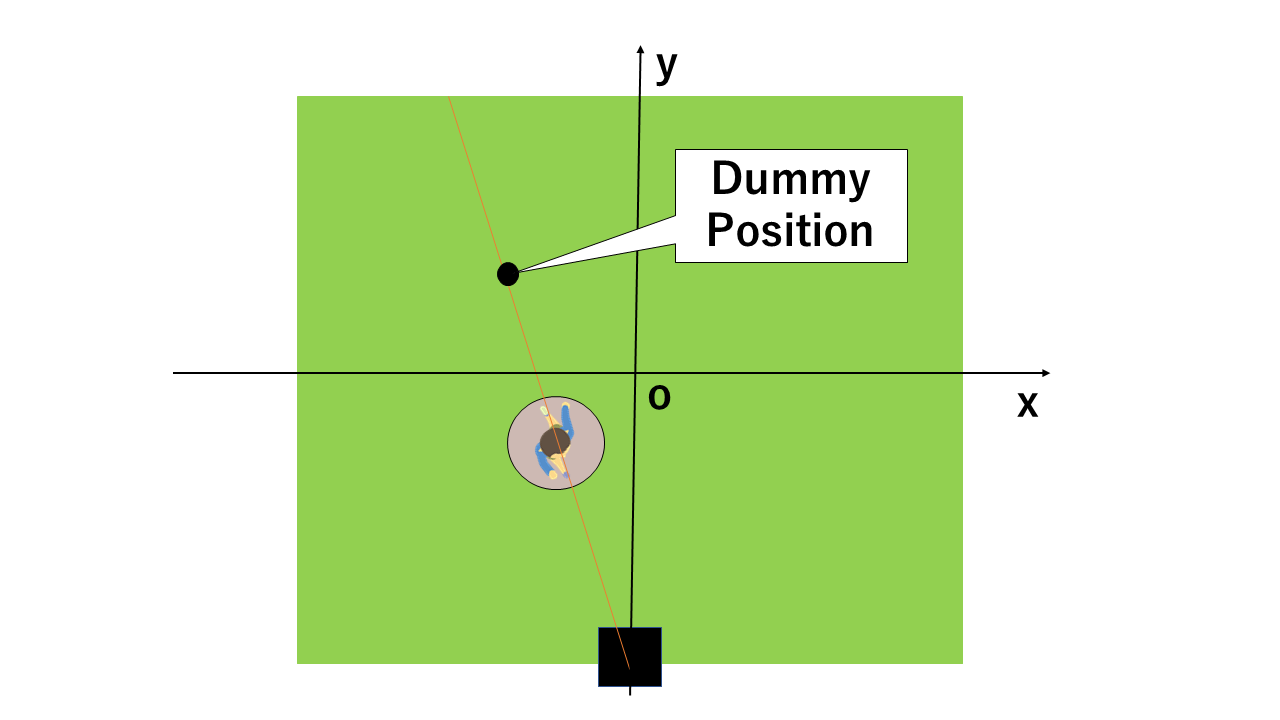
\includegraphics[width=\linewidth, clip]{./figure/chapter3/dummy.png}
    \caption{Dummy Position}
    \label{fig:dummy}
\end{figure}

\cref{eq:occlusion}の方程式より境界の座標を代入することにより交点の座標が求められる.
1人の人物に対して1つのダミーが生成されるためダミーを含めた人物の数は,
LiDARが認識している人物の数を$n$人とすると,撮影ベクトルを付与される人物とダミー人物の合計の数は$2n$となる.

\newpage
\section{複数LiDARでの人物認識}
LiDARを複数使用して人物認識を行う場合,それぞれのLiDARでとらえた物体を同一の座標系に合わせる必要がある.
この別々に認識された物体を1つの座標系にマージする際,同一人物を別の人物として捉えてしまうと
不必要な撮影ベクトルが存在することになり効率の悪い撮影計画になる.

\begin{figure}[b]
    \centering
    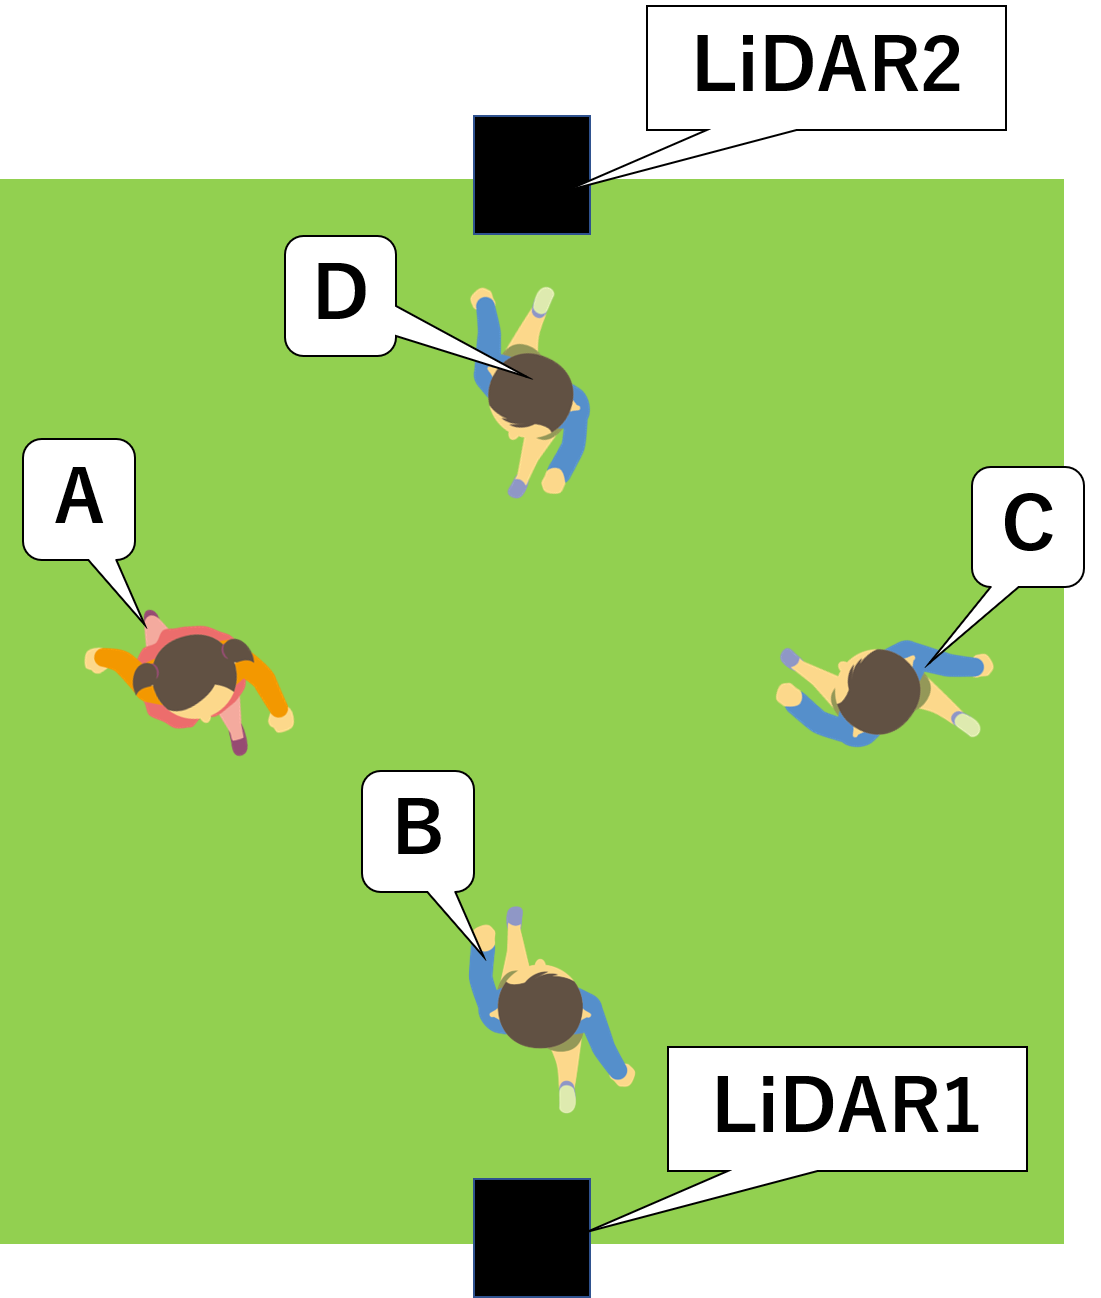
\includegraphics[width=0.7\linewidth, clip]{./figure/chapter3/example.png}
    \caption{Example of Person Recognition}
    \label{fig:example}
\end{figure}

\begin{figure}[p]
    \centering
    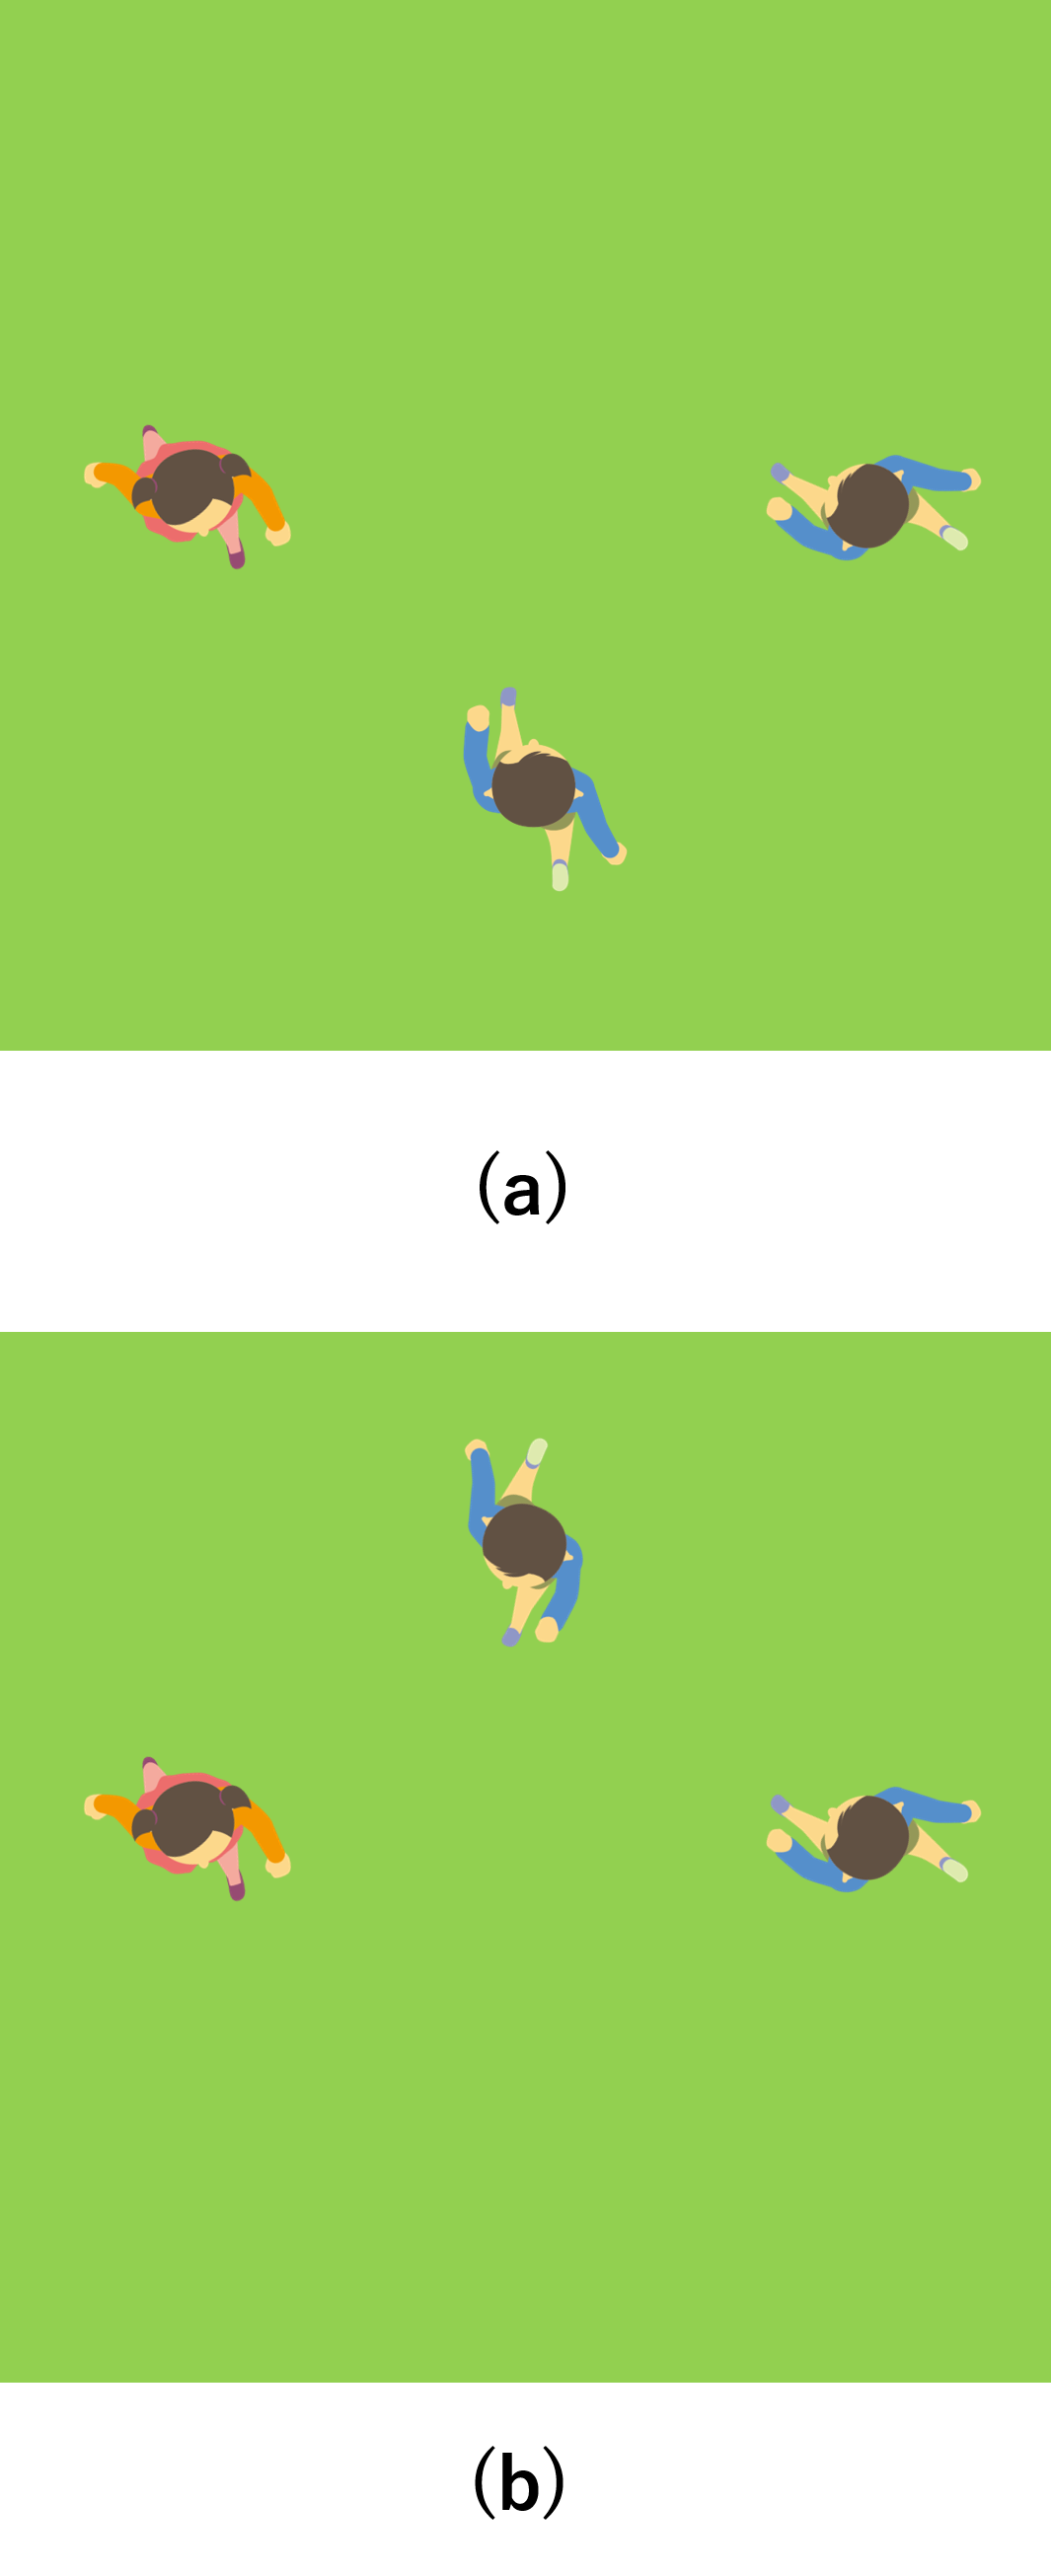
\includegraphics[width=0.5\linewidth, clip]{./figure/chapter3/recognized_person.png}
    \caption{Person recognized by LiDAR1 or LiDAR2}
    \label{fig:person_recognized}
\end{figure}

\newpage
例として\cref{fig:example}のような人物とLiDARの配置を考える.
4人の人物それぞれにA,B,C,Dのラベルを割り振る.
前節で述べていたオクルージョンエリアをLiDAR1,LiDAR2についてそれぞれ考慮すると,
人物DがLiDAR1のオクルージョンエリアに配置されていて,人物DがLiDAR2のオクルージョンエリアに配置されている.
人物A,Cは両方のLiDARから認識することができる.
LiDAR1が認識できる人物を\cref{fig:person_recognized}(a),LiDAR2が認識できる人物を\cref{fig:person_recognized}(b)に示す.
2つのLiDARの認識している人物をそのままマージすると人物A,Cが重複して数えられることになる.

\subsection{重複人物のマージ方法}
2つのLiDARで同一人物を認識するとき,\cref{fig:example}の人物Aを例として考えると,
LiDAR1は人物Aの前面,LiDAR2は人物Aの背面を認識することになる.
この認識のずれにより,それぞれのLiDARが認識した点群から生成される円の中心座標が完全一致する可能性は限りなく低いと考えられる.


\section{地形情報の構築}
.


\section{本章のまとめ}



\end{document}
